\chapter{Background}
\label{cha:background}

The chapter covers practical and theoretical knowledge necessary to understand further reading and evaluate the drawn conclusions. It also presents different origins of several scientific ideas, which have turned to be similar to each other.
%---------------------------------------------------------------------------
\section{General programming concepts}
\label{sec:programmingConcepts}

Computer science and programming are relatively green fields of science in comparison to other contenders. The first computer program was probably written between 1842-1843 by Ada Lovelance in order to calculate Bernoulli numbers. The script was supposed to run on the Analytical Engine - the mechanical predecessor of what we today call a computer \cite{history}. However, the real growth of the discipline started after the creation of Alan's Turing "a-machine" which, as one of the firsts, enabled execution of stored programs \cite{history}. From that time, progress was enormous. Nevertheless, some vital concepts remain unchanged. After all new inventions, programs still are composed of selections, iterations, sequences and in directions.

According to Robert Martin \cite{cleanArch}, two discoveries were milestones in the history of computer science. The first was the introduction of compilation and programming languages. The second was the establishment of paradigms.

Programming paradigms are models to follow when designing software. There are three: 
\begin{itemize}
\item structured
\item object-oriented
\item functional
\end{itemize}
When examined (as is presented in \textit{Clean Architecture} \cite{cleanArch} their reason is not to provide new ways of programming, but to create the restraints on code. Specific restrictions are covered in following subsections. 

% TODO!
% sources: Wikipedia

\subsection{Structured Programming}
\label{subsec:oop}

The structured programming paradigm is the rarest mentioned one. Some developers take it as something granted, due to how obvious these rules appear. However, in the past, it was not always so. 
The paradigm was introduced by, one of the fathers of the discipline, Edsger Wybe Dijkstra. He found that free use of code jumps (e.g. goto expression) should be restricted due to the massive amounts of errors it produced. In order to conduct that, he introduced loops and control flow statements in the form as they are known today (for, while, if, else, switch) in most languages. 

Structured programming is all about structuring the direct flow of control  \cite{cleanArch}. 

\subsection{Object Oriented Programming}
\label{subsec:oop}

Object-oriented programming is mostly known as a way of data as objects. That is true, but the most crucial part is about inverting the flow of control. Before object-oriented paradigm programming was treated as writing lines of code, that executed consecutively. Applications had to be designed from the beginning (start of execution) to an end. The paradigm enabled treating parts of code as separate modules (objects with the desired behaviour), which with the specified interface, can be developed independently and be easily plugged in.

Object-oriented programming is all about structuring and restricting the indirect flow of control \cite{cleanArch}.

%source: clean architecture

\subsection{Functional Programming}
\label{subsec:functionalProgramming}

The functional paradigm is the oldest one. It has its root in mathematics. This approach notices the problem of data mutation and restricts it \cite{cleanArch}. Once assigned, the variable should never be assigned again. The thing that is passed with flow control should not be variables, but only their values or behaviour (functions). 

Functional programming is all about restricting variable allocation  \cite{cleanArch}. 

\subsection{Queue}
\label{subsec:queue}

As programs started to be more and more complicated, a need for grouping of multiple variables became a necessity. Thus a lot of data structures were introduced. Like with any problem in computer science, there is no the best data structure to support all use-cases. Each has a different application.

One of them is a queue. This paper describes it because the implementation of RabbitMQ is based upon it. 

A queue is a simple structure that stores data. It is of type FIFO (the first element in is the first out). A good analogy is a physical queue. All typical operations supported are:
\begin{itemize}
\item push/enqueue - add the bottom element to the queue (at the end of it) 
\item pop/dequeue - remove the top element from the queue (from the beginning of it) 
\end{itemize}

An element of the queue has to be taken from the beginning of it in order to be read. That is the only way to read an element. It is not possible to access elements inside the queue. 

An element can be added only to the end of the queue. 


\begin{figure}[h!]
 \centering
  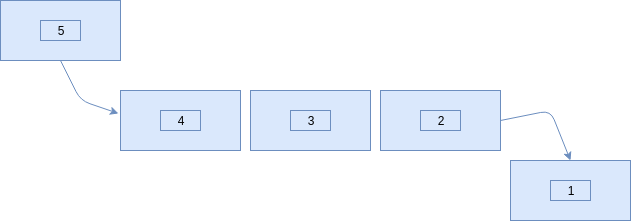
\includegraphics[width=0.8\textwidth]{pictures/que.png}
  \caption{Visualisation of a queue}
  \label{fig:queue}
\end{figure}


\subsection{Append log}
\label{subsec:log}

Most people recognise log as a text file, written by a certain program. That is a correct association because log files are the most common implementation, but the log is much more. It is a data structure. Not the obvious one, but definitely the simplest one. The only supported, possible operations are:
\begin{itemize}
\item append
\item read element
\end{itemize}
Items in a log cannot be modified and always preserve the order. The only way to modify its structure is to append an item to the end of it. Records when read always preserve an order. 

\begin{figure}[h!]
 \centering
  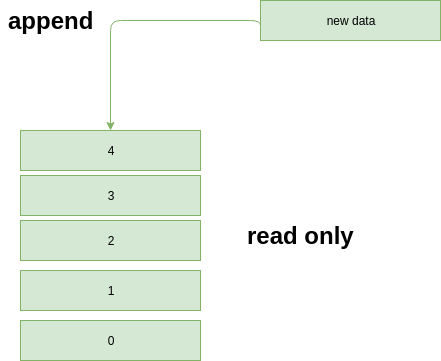
\includegraphics[width=0.8\textwidth]{pictures/log.png}
  \caption{Visualisation of an append log}
  \label{fig:log}
\end{figure}


%source:" I <3 Logs"

\subsection{State and behaviour}
\label{subsec:stateAndBehaviour}

The state is a value of remembered operations held by a program in memory. Behaviour is operations performed by the program. It is common to identify a  state as variables and behaviour as functions/methods.

Recently there was a huge trend to create stateless programs and tap into functional programming. A state is nothing wrong by itself, but it brings many risks, e.g. modifying the same resource concurrently. There are many ways to prevent it, e.g. thread-safe structures, atomic operations, locks, usage of databases. 

One of the solutions to the mentioned problem is to follow a functional paradigm. Its remedy is simple - not use a state at all. Every information that is supposed to be passed within the application should be done so in the form of behaviour, not variable.

%-------------------------------------------------------------------------

\section{Idempotence}
\label{idempotence}

Idempotence is the property, which is a critical concept in functional programming. 

Method, function or mathematical operation is idempotent if given the same input parameters always produces the same results. 

Examples of idempotent and not idempotent methods are presented on the listing below.
\begin{itemize}
\item function, that takes two integer values and returns their sum is idempotent. For example, 2 + 2 always equals four, 
\item function that given new value and an address in memory, replaces the value with the new one is idempotent,
\item function, that takes an existing pointer to the memory, increments its value by 1, returns the result is not idempotent. Every function call will increase its value.
\end{itemize}

The most significant gain of the idempotent method is that in case of unexpected error during execution (for example, lost connection), method call can be retrieved as many times as necessary. 


%source: webster dictionary https://www.merriam-webster.com/dictionary/idempotent
%-------------------------------------------------------------------------
-
\section{Data Storage}
\label{subsecdataStorage}
Many words had been spoken on the topic of data in the 21st century. After all, what the most programs do is reading data in one format, modifying it, sending or storing somewhere in a different format. There is the reason why the term computer science is often used interchangeably with information technology. It is obvious that with the massive production of various information, there is a need for efficient ways of storing it. 


\subsection{Types of data storage}
\label{subsec:typesOfDataStorage}
Data can be stored in many various ways. It does not have to be digital information saved on a hard drive. Pens and paper are also devices that can be used. This thesis highlights several concepts regarding data that are necessary to understand how message brokers work.

Digital data can be stored locally and remotely. There are different types of physical memory devices. Some are volatile; some are not. Using volatile memory is much faster and more efficient, but it will not preserve the information forever. 

\subsection{Filesystem and databases}
\label{subsec:filesystemAndDatabases}

Hardware needs software to manage its resources. Memory is one of them. A program responsible for that is usually called an operating system. For example, the Linux kernel manages over processes, memory and hardware devices. Traditionally to access a persistent memory (e.g. hard-drive), typically operating systems provide a filesystem. As the name suggests, in this approach, data is organised in files. It brings many advantages. It is efficient, simple, safe (different users have different permissions), thread-safe (usually operating system provides locking) and easy to migrate in the future. However, the usage of files has a lot of significant flaws, which are not to be overcome. There are no ways to handle:
\begin{itemize}
\item redundancy - duplication of a single piece of data, which leads to inconsistency; 
\item sharing - a file cannot be shared among the users, or it is complicated;
\item concurrency - a single file can be read by a single user at a time;
\item efficient searching - files can only be scanned line, byline; 
\item integrity - a way to verify data, before modification of a file
\end{itemize}
% source: https://developer.ibm.com/articles/l-linux-kernel/

In order to accommodate these problems, database management systems (DBMS) and relational database management systems (RDBMS) were introduced. RDBMS structure data into tables of records and introduce relations between them. Example of a relational database is MySQL, PostgreSQL, SQLite. 

% TODO.

\subsection{Transactions, ACID and isolation levels}
\label{subsec:acid}

Atomicity, Consistency, Isolation, Durability (often referenced as acronym ACID) are the requirements that all database systems try to achieve. Some of them do, some do not. All the rules regard transactions. 

\begin{itemize}
\item Atomicity - Either all operations within a single transaction are executed or no 
\item Consistency - There is no half-completed transaction in the entire system, transactions cannot violate the rules of the system,
\item Isolation - Transactions are isolated from each other - they have no access to any resources the other one posses,
\item Durability - Once a transaction is completed, it cannot be undone. The state is modified and will be persisted upon any failures (system, connection, ec.), 
\end{itemize}


% source ACID vs BASE: The Shifting pH of Database Transaction Processing
% https://www.dataversity.net/acid-vs-base-the-shifting-ph-of-database-transaction-processing/#


\subsection{Read and write efficiency}
\label{subsec:rwEfficiency}

Since the beginning of databases, never-ending debate exists, whether to use read-efficient database (usually normalised) or write-efficient database (denormalised). It is true, indeed, that optimisation of a source of data (on the software level) in one-way decreases performance in the other. For example, structuring (normalisation) data makes it more difficult to read and vice versa. 

This problem is severe. It seriously slows down many systems. The widely accepted answer to that is the use of different data sources each optimised in another way (one for writes, one for reads, one for any other application). It is not an easy to implement and clean solution. Moreover, it forces developers to commit one of the most severe crimes in programming, which is data duplication.

As the approach is difficult, it requires special tools. One of them is, deeply covered in this thesis, Apache Kafka. Also, the book "Making Sense of Stream Processing" \cite{streams} discusses this problem sincerely.



\subsection{Cache}
\label{subsec:cache}
Depending on the location and method of storage, some pieces of data are more inconvenient to access than the others. Also, most solutions are either efficient for reading or writing (there is always a consensus). In order to accommodate these problems, a technique of caching is used very often. 

Caching data, in most cases, refers to saving an inefficient to retrieve data in more volatile memory (e.g. RAM). It provides quick access to frequently used parts of information and increases performance. However, doing this is as dangerous as it looks because of the data duplication. 


%--------------------------------------------------------------------------
\section{Unix approach}
\label{sec:unixApproach}
The community of programmers and the industry are wide open to all innovations. That is not a surprise. New technologies can bring tremendous advantage over the competition. However, leaning towards new and shiny tools may cause forgetting the past solutions and reoccurrence of the old problems. 

The problem of communication and data distribution between different entities was present a long time before the microservices architecture \cite{streams}. The thesis covers how the Unix systems handle it in this section. 

\subsection{File}
\label{subsec:file}
In order to handle complicated operations, UNIX systems bring an easy to use abstraction. Everything is a file. Furthermore, a file is the stream of bytes, which can be written to and can be read. Not only data is stored in the files in a filesystem. Also, all the devices, ports and processes are visible as a file. Sending a piece of data over the web means writing it to the specific port (visible as a file/stream of bytes). 

\subsection{Process communication}
\label{subsec:processCommunication}
One of the main tasks of all operating systems is handling the execution of different processes simultaneously. The problem of communication between processes occurred when people came up with the idea of parallelisation of a single task into multiple processes. It was much before the first distributed platforms. 

The UNIX systems are examples. There are many ways to provide this functionality. Some of them are messaging ques, shared memory and semaphores \cite{linuxDocs}. In order to understand the subject of this thesis, the most important are pipes. 


\subsection{Pipes and tools}
\label{subsec:pipesAndTools}
Linux pipes are one of the most loved by developers features of this operating system. Many of the users think of pipes as a way to pass the output from one command to another, like in the code listing below:
\begin{verbatim}
$ command1 | command2
% or
$ command1 > command2
\end{verbatim}
Moreover, they are right, but what it is needed for and what the pipe is? Shouldn't the kernel handle communication and take the output from one application and pass as an argument to another? 

The answer is simple. The pipe can be compared to the real pipe and bytes stream to any stream. As soon as the first piece of data is processed by the first command, it is sent to another. There is no need for waiting for the rest of the arguments to be processed. The first process does not have the information about the destination the data is sent. The receiving process does not have information about the origin of the incoming data. 

\begin{figure}[h!]
 \centering
  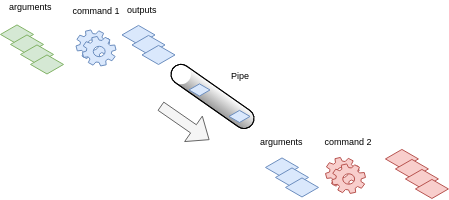
\includegraphics[width=0.8\textwidth]{pictures/stream.png}
  \caption{Visualization of unix pipe }
  \label{fig:stream}
\end{figure}


These characteristics simplify the programming of particular command-line tools. It creates a specific interface and abstraction. It is worth noticing the same characteristics are often described as the main benefits of object-oriented programming and microservices. The difference is, the concept is much older. 

%--------------------------------------------------------------------------
\section{Cloud}
\label{sec:cloud}

Cloud is one of the hottest topics in the whole industry. Despite the popularity of the word, it is not always clear what does it mean. Regardless of its frequent use as another buzzword in the marketer's collection, it is an important programming concept. This section of the thesis describes what cloud computing is explicit. The concept is one of the critical reasons for the existence of microservices architecture.

\subsection{Cloud abstraction and definition}
\label{subsec:cloudAbstraction}

With high generalisation, the cloud is often understood as many computer machines (servers) working as one. Although it is not a correct definition, it describes how a cloud can be thought of and is not entirely wrong.

Following the article on Amazon Web Service web-page (one of the largest cloud providers): "Cloud computing is the on-demand delivery of computing power, database, storage, applications, and other IT resources via the internet with pay-as-you-go pricing." \cite{aws-cloud-computing} 

Also, the following characteristics can be specified\cite{cloud-computing}:
\begin{itemize}
\item On-demand self-service - Computer services so as applications, devices or a network can be granted as needed \cite{cloud-computing}.
\item Broad network access -  Services are available over the Internet and reached through various devices \cite{cloud-computing}.
\item Resource pooling - Physical resources are available to the consumer dynamically. Resources currently being used can change regarding consumer needs \cite{cloud-computing}.
\item Rapid elasticity - Cloud Capabilities can be easily selected and discharged automatically. The cloud capabilities are accessible to the user in any number at any moment \cite{cloud-computing}.
\item Measured service - Cloud systems automatically manage and optimise resource usage by measuring costs of use \cite{cloud-computing}.

\end{itemize}

\subsection{Scalability}
\label{subsec:scalability}
Scalability is another concept that does not have formal definition\cite{scalability}. Even with many tries to formalise it, it is not a comparable metric. However, it is one of the key concepts in order to understand the reasons to use message brokers.

To follow further reading understanding the next sentence is sufficient. The scalable system does not decrease its performance significantly (e.g. in terms of speed of processing requests) when exposed to the increased load of requests. In other words: the scalable system can respond to dynamically rising amount of users, and its performance will not decrease significantly. 

The two standard methods of scaling are horizontal scaling and vertical scaling. Vertical one means increasing the computing power of a single machine. Horizontal scaling means increasing the number of machines working on the same process. It is easy to conclude, vertical scaling is much easier to utilise. Horizontal one requires special programming (code has to be written with parallel execution in mind). However, vertical scaling hits its limit very soon because of technological constraints. 

\subsection{Load balancing}
\label{subsec:loadBalancing}

Load balancing is the vertical scaling technique of distributing the loads between many computing devices (which usually perform identical tasks). It is an old concept. However, with the introduction of a cloud, it is one of the important ones. Computing devices may be computers, a computer cluster, network links, central processing units, disk drives or services.

Load balancing requires individual module responsible for handling it. Equal distribution of load between workers is the mathematical problem. There are many algorithms called scheduling algorithms which are used to determine a receiver of the request. Their purpose is to provide equal distribution, which often is not a trivial problem. That happens, because an interval between messages and time of handling each by the worker may vary.  

In order to understand the primary goal of the thesis, this concept is critical. However, the dilemma of choosing load-balancing algorithms and in-depth knowledge of mathematical problems is beyond the scope of this document. More can be found on research "Performance tradeoffs in static and dynamic load balancing strategies" published by NASA \cite{load-balancing}

\begin{figure}[h!]
 \centering
  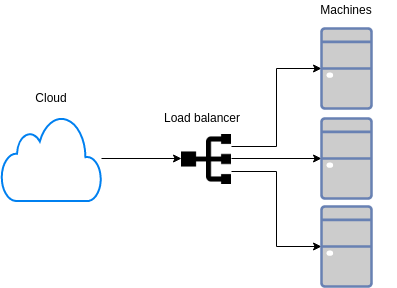
\includegraphics[width=0.8\textwidth]{pictures/loadbalancing.png}
  \caption{Visualization of load balancing }
  \label{fig:load-balancing}
\end{figure}


\subsection{Virtual machines}
\label{subsec:vm}

The introduction of virtual machines was the events that shaped how the whole internet industry works today. Virtual machines introduced another level of abstraction and enable the foundation of what we today call a cloud. 

Popek and Goldberg coined the term virtual machine in their work "Formal Requirements for Virtualizable Third Generation Architectures" \cite{VM}. They described it as "an efficient, isolated duplicate of a real computer machine". Currently, people prefer to think of it as a piece of software. 

The simplest definition of a virtual machine does not sound very astounding. It is an emulation of a computer system. In other words, it is a software that provides the functionality of the other computer. The most straightforward application of this kind of tool is to run programs written for the other kind of platform (e.g. running Windows program on Linux operating system). However, there is much more to it.

There is a possibility to run several virtual machines on a single host. That is the factor that creates the most significant difference. Large web platforms usually consist of many smaller services. Deploying each service on a separate physical machine would require to take tremendous costs.

\subsection{Containers}
\label{subsec:containers}

Virtual machines have many advantages which are impossible to bypass. However, employing them requires a lot of computing power. It is, after all, installing a new operating system inside an operating system and this kind of software is typically the most heavyweight of all applications. 

In order to solve this problem, the containers were introduced. The common understanding of them is as lightweight virtual machines. It often works (containers and virtual machines have similar properties), although it is not entirely correct. A container is also a simulation of a different operating system. However, it is only a proxy. It does not install all software, that specific system consists. It uses the same modules as the host system and pretends they are from another source. Container engine is the program that enables running containers. It also manages access to specific resources (e.g. resources in term of Linux operating systems are a memory, computing power, processes and hardware devices \cite{kernel-anatomy}). 

The figure below shows the differences between containers and virtual machines. It shows the systems running three containers and three virtual machines with the same applications.

\begin{figure}[h!]
 \centering
  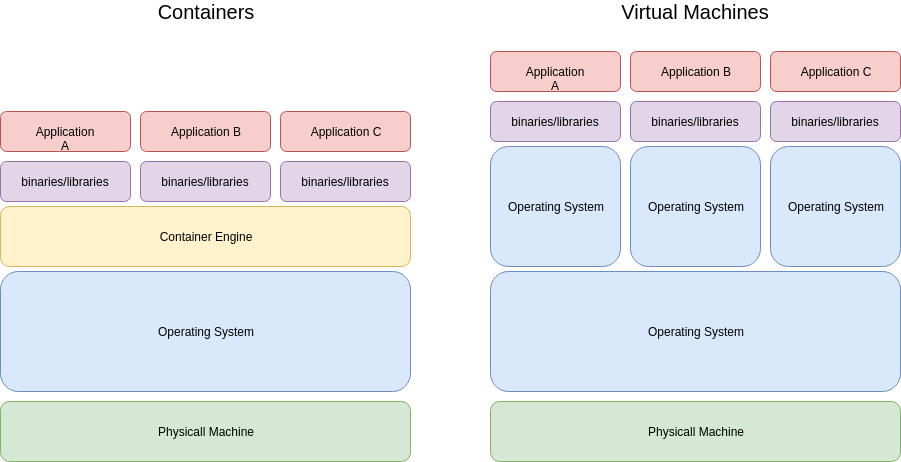
\includegraphics[width=0.8\textwidth]{pictures/containers-vs-vms.png}
  \caption{Differences between containers and virtual machines}
  \label{fig:load-balancing}
\end{figure}


\subsection{Orchestration}
\label{subsec:orchestration}

Linking previously introduced pieces of information - a cloud enables to treat many physical computer machines as one. Virtual machines enable to treat single, powerfull computer machine as many. Containers tremendously reduce the cost of running virtual machines. That facts enable designing software in a service fashion. It is no longer an issue to run any number of services on any number of physical machines. The abstraction separates both layers.

That enables dynamic orchestration. Depending on traffic passing through each service, a piece of software called orchestrator (e.g. Kubernetes) will employ the necessary number of workers (services) to execute the task. That will ensure the optimal use of available resources. 


%--------------------------------------------------------------------------

\section{Distributed programming, parallel execution and software architecture}
\label{sec:distributedProgramming}

As time progressed, it grew self-evident that the benefits of the cloud, dynamic scaling and orchestration are enormous. There is no other simple way to create scalable software, which can withstand traffic coming from millions of users. All of the major web companies moved their platforms to the clouds. 

However, no technology comes without a cost. Building an application in a modern, distributed fashion requires a different design. The cloud resources (hardware) are distributed over the network. Thus, when an application consists of many modules, they are also usually distributed over the network. This kind of software needs to be designed with the ability to handle communication errors in mind. 

\subsection{CAP theorem}
\label{subsec:capTheorem}

Brewer's CAP Theorem regards data in the distributed system. It is important to note that network connection always may be fallible - there is no guarantee one packet will reach its destination. Theorem stands that in the distributed system (understood as many connected nodes spread over a network) "it is impossible for a web service to provide the following three guarantees" \cite{cap}:

\begin{itemize}
    \item Consistency - Every data read guarantees that the data will come after the latest write
    \item Availability - Every read guarantees that data will be delivered in the reasonable amount of time (e.g. no timeout will appear)
    \item Partition tolerance - more than one partition of the system occurs
\end{itemize}

Partitioning application means that there is more than one source of data. In order to guarantee consistency, there is a necessity of synchronising application, but that may lead to timeout errors. The only way to provide the highly available and consistent system at the same time is not to partition it at all. 


\subsection{Monolith}
\label{subsec:monolith}

The thesis intends to examine the communication between services. Monolithic design is precisely the reverse style. Nevertheless, in order to understand the benefits and difficulties of microservices, it is essential to know the alternative. 

A monolithic system is built as a single entity. An application regularly consists of client-side (frontend), server-side (backend) and some type of database. Server-side is a monolith. It is responsible for executing domain logic, handling request, populating HTML and performing database commands. 

A monolithic design can also be successful. Engineers often disregard it. Nevertheless, the well-built monolith can serve its purpose (as all design patterns). It is worth noting that monolithic application also can be scaled horizontally, by replicating itself. Though, it also multiplies redundant components \cite{microservices}.
%source: https://martinfowler.com/microservices/

\subsection{Micro-services}
\label{subsec:microservices}

Microservices is the pattern of building a large scale application. It implies breaking the extensive system into many tinier services interacting with each other. It produces many advantages, yet also many not trivial to handle challenges. The thesis touches solving one of them, which is communication. Nonetheless, there are many others, which are beyond its scope.

It is critical to note that the concept of microservices has not been discovered or suddenly reported in groundbreaking research. It evolved through time, based on the work-culture of significant enterprises in the industry\cite{building-microservices}. One of the causes for that was the growing disappointment over monolithic applications. Microservices answer some technological obstacles, but the crucial is solving of organisation issues. Nowadays, the main factor which stimulates technology is business and precisely the interests. Reducing development time and optimising the organisation leads to higher profits. 

Following Sam Newman:
\begin{displayquote}
"Many organisations have found that by embracing fine-grained, microservice architectures, they can deliver software faster and embrace newer technologies. Microservices give us significantly more freedom to react and make different decisions, allowing us to respond faster to the inevitable change that impacts all of us."\cite{building-microservices}.
\end{displayquote}

From the technical viewpoint, the essential factors are the resilience, fault tolerance and capability to easily scale-out such applications. Also, the architecture grants autonomy to choose the technologies in frames of one service.

\subsection{Domain Driven Design}
\label{subsec:ddd}

Domain-driven design is the name of an approach to the making of software. It supports principally to control large and complex difficulties of massive scale. It is frequently applied alongside microservices architecture, although it produces another layer of abstraction between code composition and the physical deployment. Eric Evans started this concept in his work "Domain-Driven Design: Tackling Complexity in the Heart of Software" \cite{dddEvans} and Vough Vernon popularised it within publications: "Implementing Domain-Driven Design"\cite{implementingDDD}, "Domain-Driven Design Distilled"\cite{DDD}.

Domain-driven design can be applied regardless of the deployed architecture (also a monolith, it does not necessarily have to be microservices). The principal intention of this strategy is to concentrate on "Domain Logic", which is the essence of what service provides. Anything else should be separated and grouped. For example, parts of the domain logic of the task-tracking application would be tasks, deadlines, and similar.  Technical aspects like database connections should not. 

Domain-driven design, like microservices, forms boundaries separating modules. Still, those are the matter of contextual boundaries \cite{DDD}. The application can still be deployed as an individual entity. The indisputable benefit of this method is that if the application is deployed as a monolith, it can be broken into micro-services without significant effort. 

In this way, the division unit is not a " service", but a "bounded-context". It is accurate to consider bounded context as a problem space \cite{DDD}. Business rules should drive the separation of code into bounded contexts. Every context should serve a different purpose. For instance, in a social platform, created with DDD rules, there would be a bounded context responsible for maintaining accounts and another one liable for managing comments. 


\subsection{Command Query Responsibility Segregation}
\label{subsec:cqrs}

Command Query Responsibility Segregation, often mentioned as CQRS, is a software design often utilised in conjunction with DDD and introduced in the next section event sourcing.

All persisted data entities (for example, events in event scheduling application) form a state of an application. This information is preserved in some fashion (e.g. in a database). CQRS, as all software patterns, does not introduce anything new. It creates restrictions to follow when creating code. This method separates requests (or methods) into two types: commands and queries. Commands are the ones that alter the state of the application (write data). Queries only retrieve the current state. 

Commands are not allowed to retrieve any information. Queries cannot write or update any data. The reason for this pattern is straightforward. It simplifies parallel processing.

\subsection{Event sourcing}
\label{subsec:eventSourcing}

Event sourcing is another method of handling the state of the application. Alternatively of persisting only the current state of an application, this approach records all modifications and saves them as a changelog. The following example of it comes from Robert Martin's "Clean Architecture" \cite{cleanArch}. In banking application instead of storing account balances, the changes to the balance are stored in an append log.

When connected with CQRS described before it is easy to notice, that all modifying data requests are labelled as commands. So, every command triggers firing an event, which is stored in an append-only fashion. 

An application does not store its current state but instead computes it from registered events. The computed state can persist afterwards, although it may cause data duplication. So, the changelog is the source of truth.

The most notable benefits of this technique are fast writes and ability to reconstruct the application state from any point of time (by replaying all events). 


%--------------------------------------------------------------------------